\documentclass[a4paper,12pt]{article}
\usepackage[indonesian]{babel}
\usepackage{graphicx}
\usepackage{multirow}
\usepackage{enumitem}
\usepackage{listings}
\usepackage{wrapfig}
\usepackage[T1]{fontenc}
\usepackage{inconsolata}
\usepackage{lipsum}
\usepackage{adjustbox}


\usepackage{color}
\usepackage[table]{xcolor}
\definecolor{mygreen}{rgb}{0,0.6,0}
\definecolor{mygray}{rgb}{0.5,0.5,0.5}
\definecolor{mymauve}{rgb}{0.58,0,0.82}
\lstset{%
    language=java,
    showstringspaces=false,          % Prevent tex replacing space to bracket in code
    frame=single,                    % Set frame around code
    backgroundcolor=\color{white},   % choose the background color
    basicstyle=\footnotesize,        % size of fonts used for the code
    breaklines=true,                 % automatic line breaking only at whitespace
    captionpos=b,                    % sets the caption-position to bottom
    commentstyle=\color{mygreen},    % comment style
    keywordstyle=\color{blue},       % keyword style
    stringstyle=\color{mymauve},     % string literal style
    numbers=left,
}

\graphicspath{ {./img/} }
\begin{document}
\title{ {\Large Laporan Praktikum}\\ Algoritma dan Pemrograman Lanjut\\{\Large Pertemuan 13}}

\author{Aldzikri Dwijayanto Prathama
    \\195410189
    \\Informatika}
\makeatletter
\begin{titlepage}
    \begin{center}
        {\huge \bfseries \@title}\\[14ex]
        
\includegraphics[scale=.8]{logo}\\[4ex]
        {\large \@author}\\[12ex]
        {\large \bfseries {SEKOLAH TINGGI MANAJEMEN INFORMATIKA DAN KOMPUTER
            AKAKOM YOGYAKARTA}}
    \end{center}


%{\large \@date}
\end{titlepage}
\makeatother
%\maketitle
\newpage
\tableofcontents
\newpage

\section{Tujuan}
Mahasiswa dapat mengurutkan data dengan metode bubble sort, selection sort
dan mengimplementasikannya dalam program.
\section{Teori}
Dalam banyak aplikasi, pengurutan menjadi algoritma yang sering banyak digunakan. Kalau kita berhubungan dengan data
yang jumlahnya besar, maka data tersebut akan mudah kita kelola kalau dalam keadaan terurut dengan suatu kunci
pengurutan tertentu. Dengan data yang sudah terurut, kita akan dengan mudah mencari data, mengelompokkan data, dan
lain-lain.

\newpage

\section{Pembahasan}
\subsection{Praktik}
\subsubsection{Praktik 1}
\begin{lstlisting}
import java.util.Scanner;

public class BubbleSort {

    public void bubbleSort(float[] larik2) {
        for (int i = 0; i < larik2.length; i++) {
            for (int elemen = 0; elemen < larik2.length - 1; elemen++) {
                if (larik2[elemen] > larik2[elemen + 1]){
                    tukar(larik2, elemen, elemen + 1);
                }
            }
        }
    }

    public static void tukar(float[] larik3, int satu, int dua) {
        float temp;
        temp = larik3[satu];
        larik3[satu] = larik3[dua];
        larik3[dua] = temp;
    }

    public static void main(String[] args) {
        Scanner masuk = new Scanner(System.in);
        BubbleSort lrk = new BubbleSort();
        float[] nilai = new float[5];
        System.out.println("Masukkan 5 buah data nilai");
        for (int i = 0; i < 5; i++) {
            System.out.print((i + 1) + " : ");
            nilai[i] = masuk.nextFloat();
        }
        System.out.println("Data nilai yang dimasukkan");
        for (int i = 0; i < 5; i++)
            System.out.println(nilai[i]);
        System.out.println("Data hasil pengurutan   ");
        lrk.bubbleSort(nilai);
        for (int i = 0; i < 5; i++)
            System.out.println(nilai[i]);
    }
}
\end{lstlisting}

\textbf{Metode Sorting Bubble sort\\}
Metode Sorting Bubble sort adalah pengurutan dengan membandingkan elemen berikutnya jika elemen sekarang
lebih besar dari elemen berikutnya maka elemen tersebut ditukar. Pada program di atas terdapat tiga method, method
bubbleSort berfungsi untuk membandingkan nilai antara elemen dengan elemen berikutnya, dan memanggil method tukar jika
elemen saat ini lebih besar dari elemen berikutnya. Method tukar berfungsi untuk
menukar nilai elemen. Dan method main yang berguna untuk memasukkan, memanggil method bubbleSort, dan mencetak hasil ke
layar.

\begin{center}
    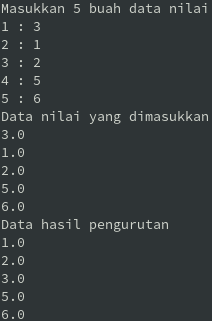
\includegraphics[scale=1]{1.png} 
\end{center}

\subsubsection{Praktik 2}
\begin{lstlisting}
import java.util.Scanner;

public class SelectionSort {

    public void selectionSort(float[] larik2) {
        for (int i = 0; i < larik2.length; i++) {
            int min = i;
            for (int elemen = i + 1; elemen < larik2.length; elemen++) {
                if (larik2[min] > larik2[elemen])
                    min = elemen;
            }
            tukar(larik2, min, i);
        }
    }

    public void tukar(float larik3[], int satu, int dua) {
        float temp;
        temp = larik3[satu];
        larik3[satu] = larik3[dua];
        larik3[dua] = temp;
    }

    public static void main(String[] args) {
        Scanner masuk = new Scanner(System.in);
        SelectionSort lrk = new SelectionSort();
        float nilai[] = new float[5];
        System.out.println("Masukkan 5 buah data nilai");
        for (int i = 0; i < 5; i++) {
            System.out.print((i + 1) + " : ");
            nilai[i] = masuk.nextFloat();
        }
        System.out.println("Data yang dimasukkan");
        lrk.selectionSort(nilai);
        for (int i = 0; i < 5; i++)
            System.out.println(nilai[i]);
    }
}
\end{lstlisting}

\textbf{Selection Sort\\}
Selection sort adalah pengurutan dengan mencari dari elemen yang berikutanya sampai dengan elemen
terakhir jika ditemukan elemen lain yang lebih kecil dari elemen sekarang maka elemen
yang bersangkutan akan ditukar. Oleh karena itu setiap langkah selalu memilih satu
baris dari baris berikutnya. Pada program di atas terdapat tiga method, method
selectionSort berfungsi untuk membandingkan nilai antara elemen dengan elemen berikutnya, dan memanggil method tukar jika
elemen saat ini lebih besar dari elemen berikutnya. Method tukar berfungsi untuk
menukar nilai elemen. Dan method main yang berguna untuk memasukkan, memanggil method selectionSort, dan mencetak hasil ke
layar.
\begin{center}
    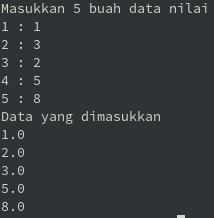
\includegraphics[scale=1]{2.png} 
\end{center}

\newpage

\subsection{Latihan}
\subsubsection{Latihan 1}
Melakukan sorting dengan menggunakan kelas Collection.
\begin{lstlisting}
import java.util.List;
import java.util.Arrays;
import java.util.Collections;

public class Sort1 {
    public static void main(String[] args) {
        String[] suits = { "Hearts", "Diamonds", "Clubs", "Spades" };

        // Create and display a List containing the suits array elements
        List<String> list = Arrays.asList(suits); // create List
        System.out.printf("Unsorted array elements: %s\n", list);

        Collections.sort(list); // sort ArrayList

        // output list
        System.out.printf("Sorted array elements: %s\n", list);
    }
}
\end{lstlisting}
Method Collections.sort(), bisa diimport dengan menggunakan java.util.Collections. Method ini berfungsi untuk
mengurutkan elemen, pada list yang ditentukan, dengan urutan naik.

\begin{center}
    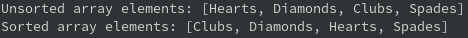
\includegraphics[scale=0.8]{3.png} 
\end{center}

\subsubsection{Latihan 2}
Sorting descending

\begin{lstlisting}
import java.util.List;
import java.util.Arrays;
import java.util.Collections;

public class Sort2 {
    public static void main(String[] args) {
        String[] suits = { "Hearts", "Diamonds", "Clubs", "Spades" };

        // Create and display a list containing the suits array elements
        List<String> list = Arrays.asList(suits); // create List
        System.out.printf("Unsorted array elements: %s\n", list);

        // sort in descending order using a comparator
        Collections.sort(list, Collections.reverseOrder());

        // output List elements
        System.out.printf("Sorted List elements: %s\n", list);
    }
}
\end{lstlisting}
Untuk mengurutkan secara terbalik dengan menggunakan method Collection, tambahkan method Collection.reverseOrder pada
saat memanggil method collections.
\begin{center}
    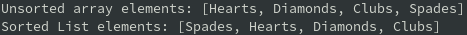
\includegraphics[scale=0.8]{4.png} 
\end{center}

\newpage

\subsection{Tugas}
\subsubsection{Insertion Sort}
Insertion sort adalah algoritma sederhana yang cara kerjanya mirip seperti mengurutkan kartu di tangan kita.
\begin{center}
    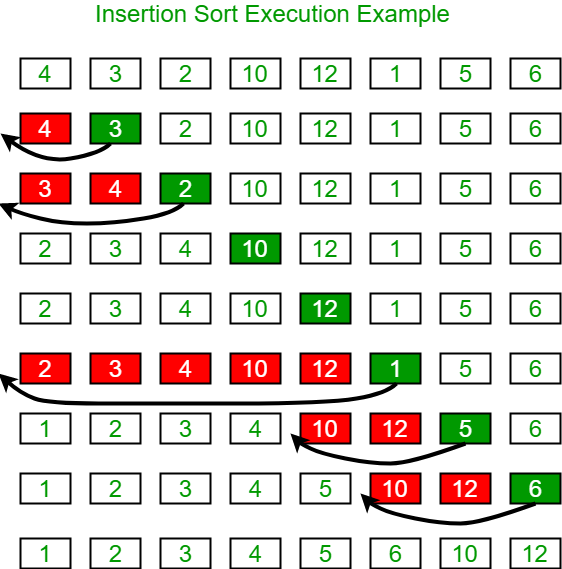
\includegraphics[scale=0.6]{insertionsort.png} 
\end{center}

\subsubsection{Merge Sort}
Prinsip utama yang diimplementasikan pada algoritme Merge Sort sering kali disebut sebagai pecah-belah dan taklukkan
(bahasa Inggris: divide and conquer). Cara kerja algoritme urut gabung adalah membagi larik data yang diberikan menjadi
dua bagian yang lebih kecil. Kedua larik yang baru tersebut kemudian akan diurutkan secara terpisah. Setelah kedua buah
list tersusun, maka akan dibentuk larik baru sebagai hasil penggabungan dari dua buah larik sebelumnya.
\begin{center}
    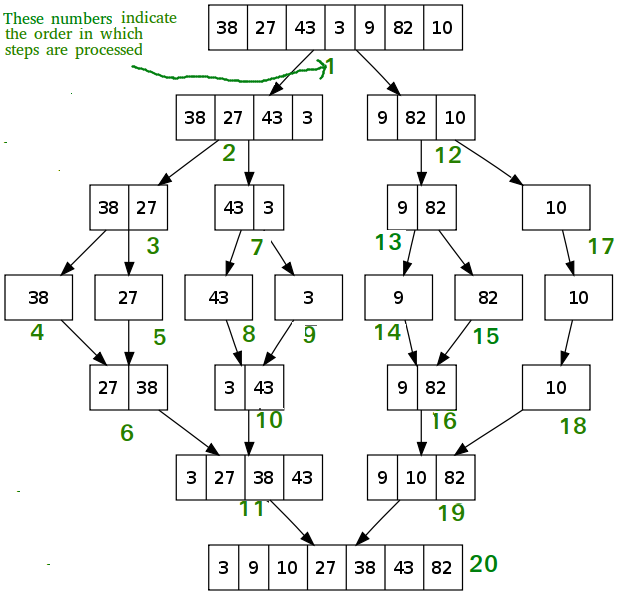
\includegraphics[scale=0.6]{Merge-Sort-Tutorial.png} 
\end{center}

\subsubsection{Quick Sort}
Quicksort merupakan Algoritme Pembagi. Pertama quicksort membagi list yang besar menjadi dua buah sub list yang lebih
kecil: element kecil dan element besar. Quicksort kemudian dapat menyortir sub list itu secara rekursif.\\

Langkah-langkah pengerjaannya seperti berikut:
\begin{enumerate}
    \item Ambil sebuah elemen, yang disebut dengan pivot, pada sebuah daftar.
    \item Urutkan kembali sebuah list sehingga elemen dengan nilai yang kecil dari pivot berada sebelum pivot, sedangkan
        seluruh element yang memiliki nilai yang lebih besar dari pivot berada setelahnya (nilai yang sama dapat berada
        pada pivot setelahnya). Setelah pemisahan, pivot berada pada posisi akhirnya. Operasi ini disebut Partition.
    \item Sub list kemudian disortir secara recursif dari elemen yang lebih kecil dan sub list dari elemen yang lebih
        besar.
\end{enumerate}
Kasus dasar dari rekusrif ialah list dari besaran nol atau satu, yang tidak perlu untuk di sorting.
\begin{center}
    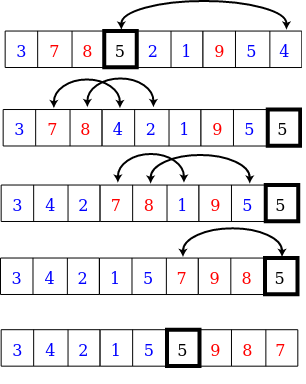
\includegraphics[scale=0.8]{quicksort.png} 
\end{center}

\newpage

\section{Kesimpulan}
Setelah praktik mahasiswa dapat mengurutkan data dengan metode bubble sort, selection sort
dan mengimplementasikannya dalam program.
\end{document}
